\subsection{Clustering with reduction vs without}
\label{subsec:clustering-with-reduction-vs-without}

This section analyses the performance of the clustering algorithms with and without reductions of the feature space.
As mentioned previously in the report, the reductions of the feature space are done by applying different
implementations of PCA. The PCA implementations are the following:

\begin{itemize}
    \item PCA via SKLearn
    \item Our own implementation of PCA
    \item Kernel PCA via SKLearn
\end{itemize}

Figures \ref{fig:clustering-results} display the results of the clustering algorithms
with and without PCA against the two datasets used, `Mushroom' and `Vowel'.
Mean of the F-measure is used to track the performance of the algorithms.

\begin{figure}[!h]
    \centering
    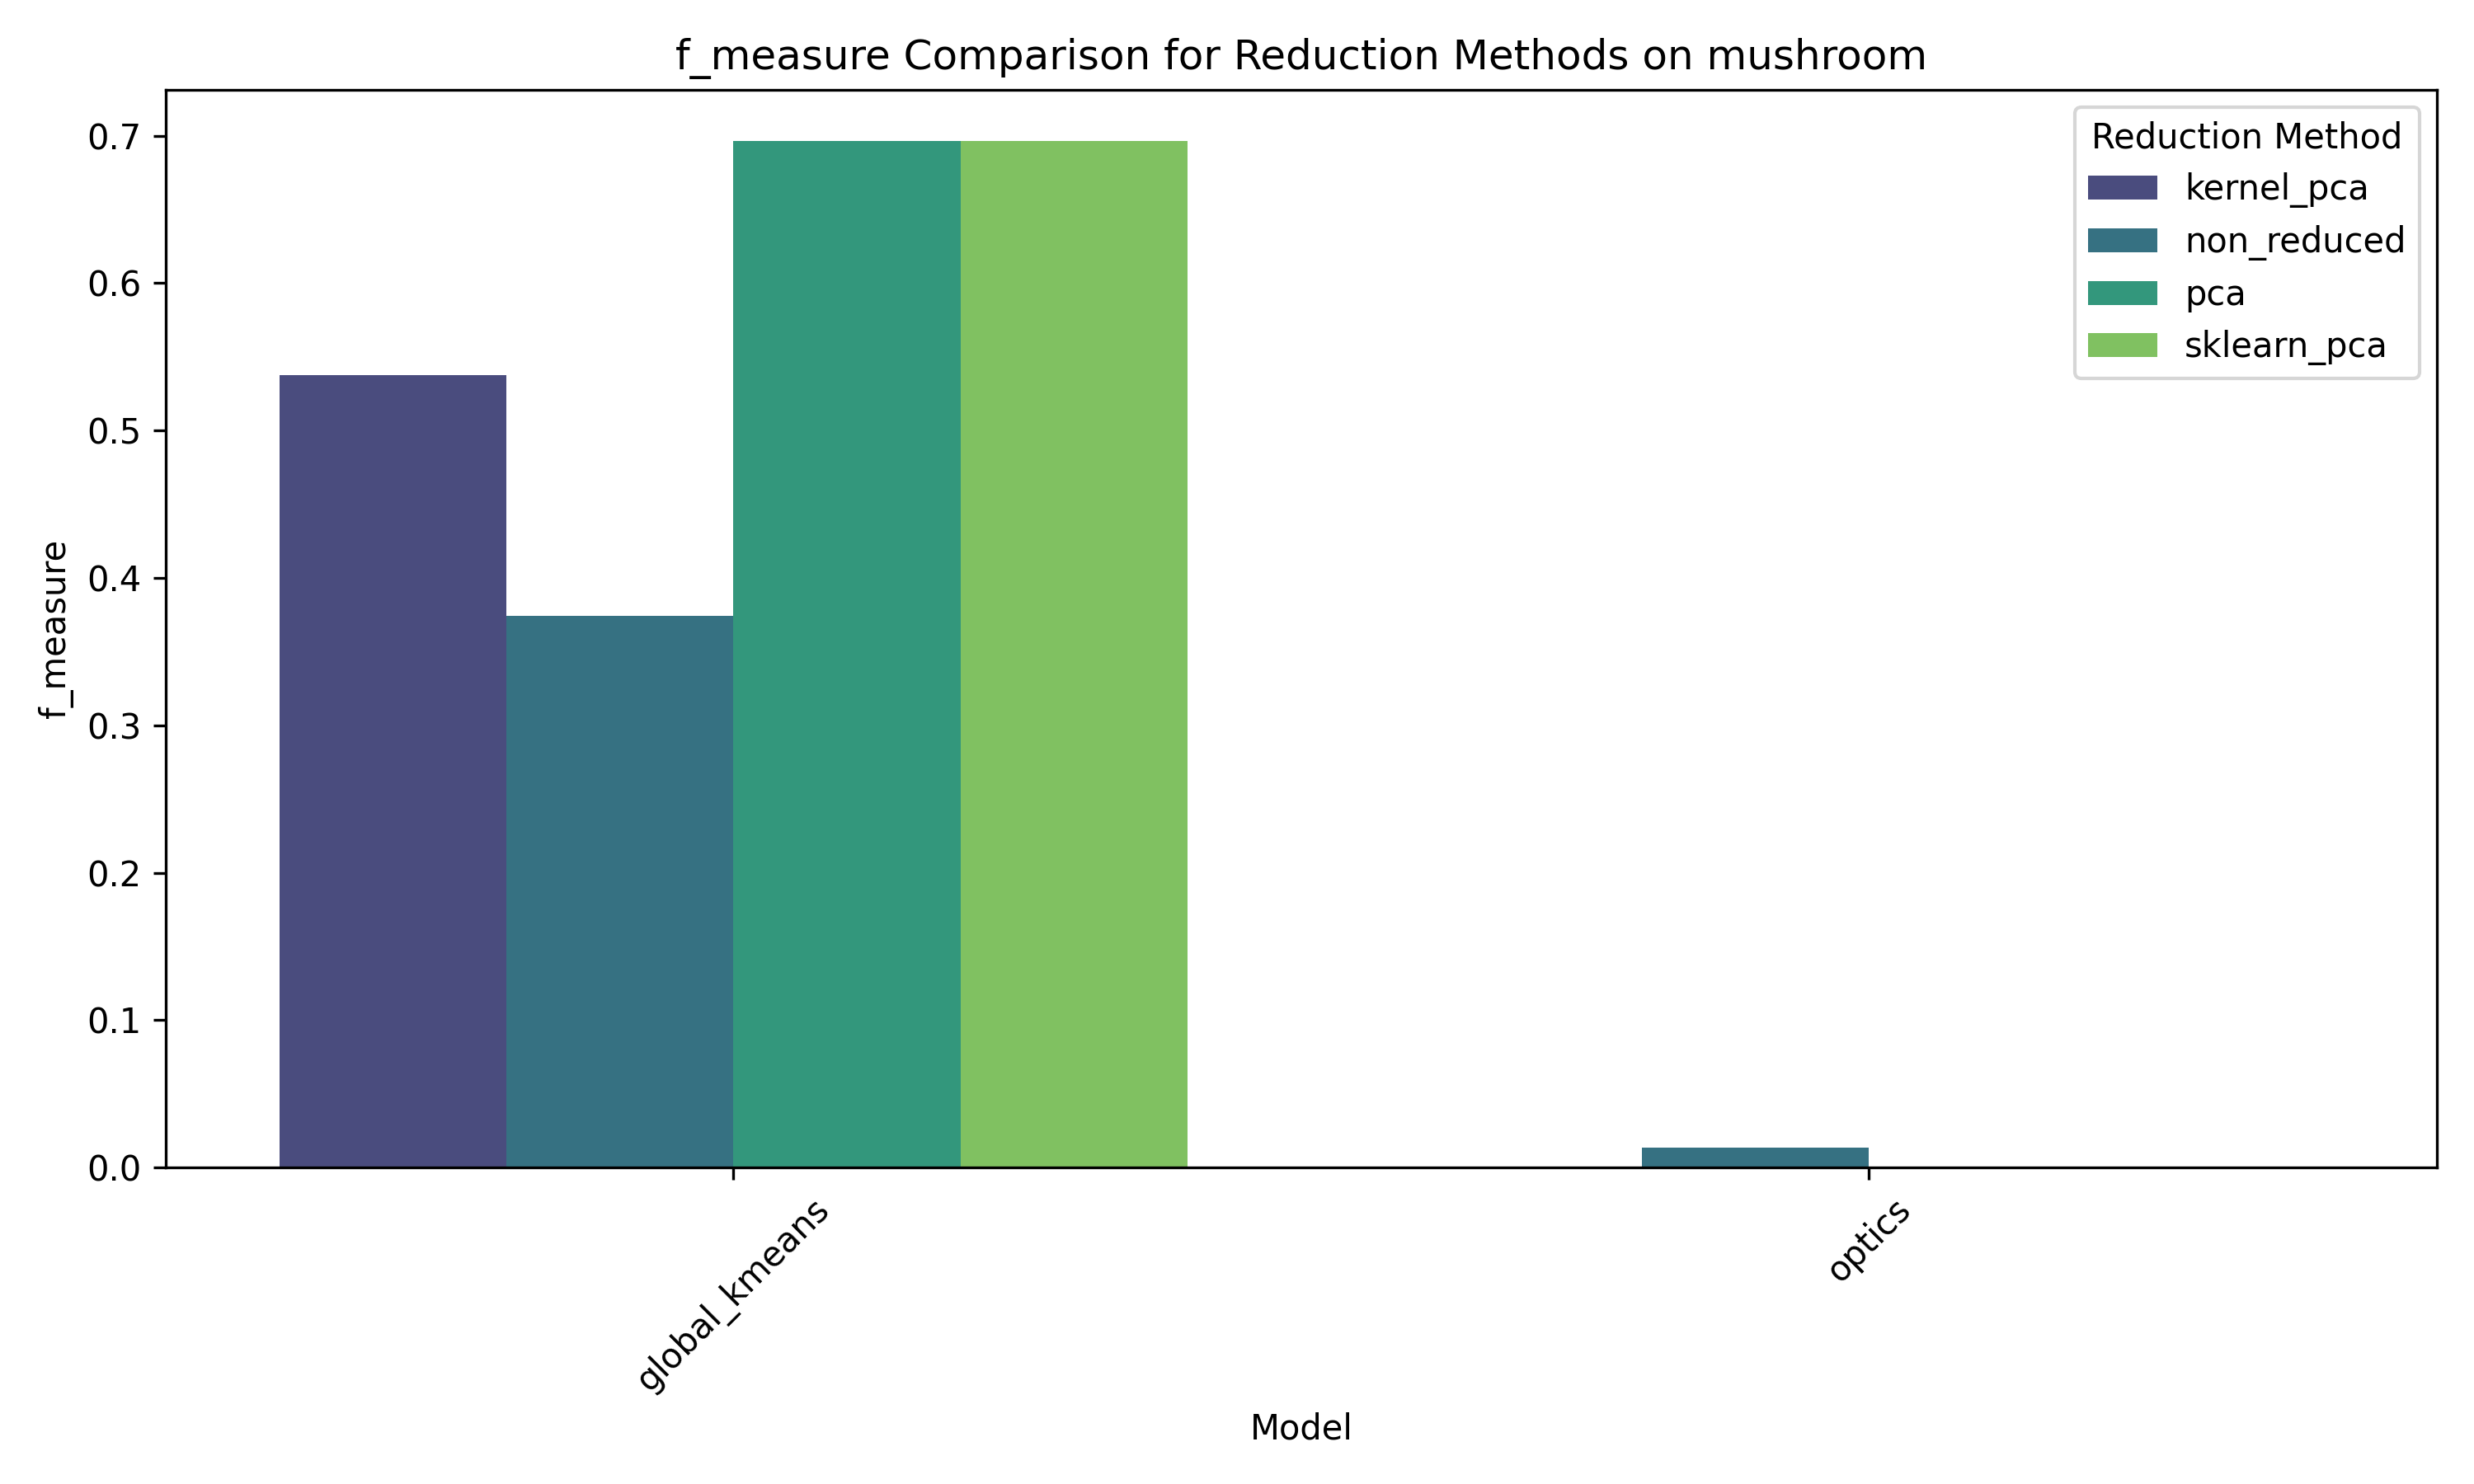
\includegraphics[width=0.45\textwidth]{figures/f_measure_comparison_mushroom.png}
    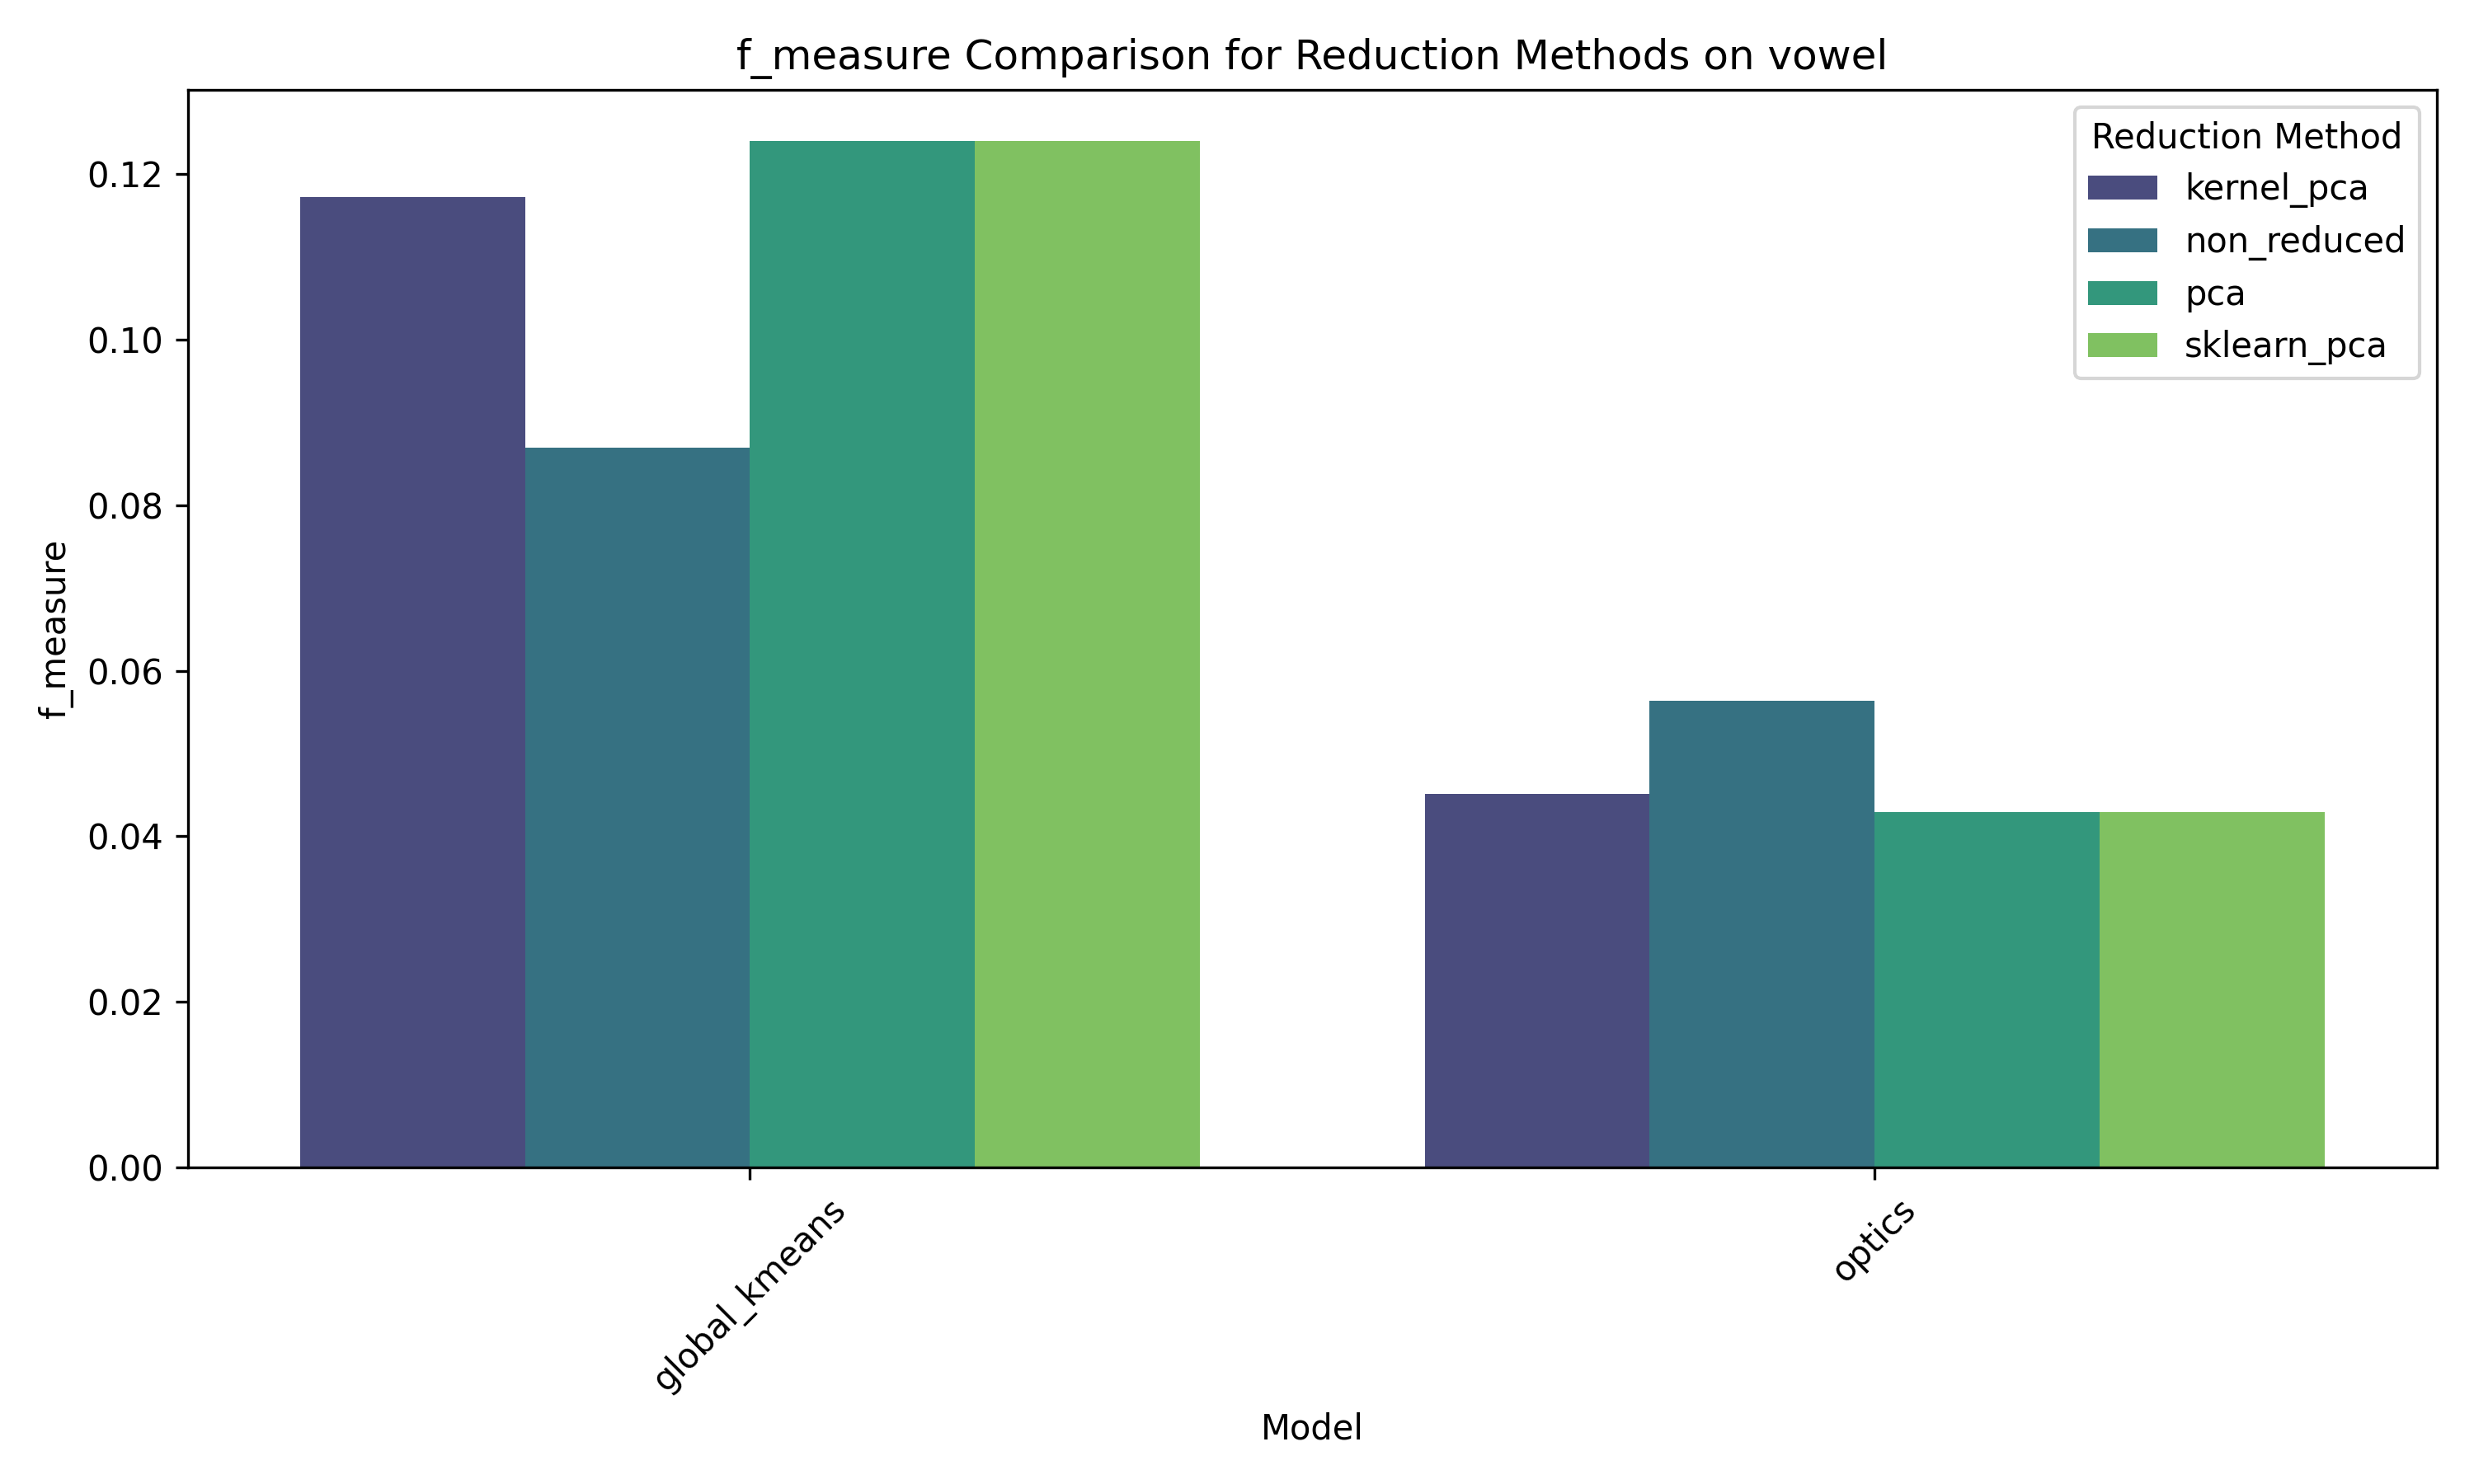
\includegraphics[width=0.45\textwidth]{figures/f_measure_comparison_vowel.png}
    \caption{Mean F-measure score with and without PCA for Mushroom (left) and Vowel (right) datasets.}
\label{fig:clustering-results}
\end{figure}


From analysing the results, it is evident that the PCA implementations generally have an 
impact on the clustering performance.

For the `Global K-Means' algorithm, each of the three 
PCA implementations have a positive impact on the clustering performance for both datasets.
On the `Mushroom' dataset, `Global-KMeans' achieves an F-Measure score of approximately 0.37
without PCA. Applying Kernel PCA via SKLearn, the F-Measure score increases to approximately 0.53. 
Our own implementation of PCA, as well as PCA vs SKLearn, achieves an F-Measure score of approximately 0.70,
which is the highest score achieved.  
A similar situation is observed for the `Vowel' dataset. Without PCA, `Global-KMeans'
achieves an F-Measure score of approximately 0.082. Applying Kernel PCA via SKLearn,
the F-Measure score increases to approximately 0.11. Our own implementation of PCA,
as well as PCA viaLearn, once again achieve the highest score of approximately 0.12.

Upon analysing the results for the `OPTICS' algorithm, it is evident that the PCA implementations
have an opposite effect on the clustering performance. For the `Mushroom' dataset, `OPTICS' achieves
an F-Measure score of approximately 0.02 without PCA. Applying any of the PCA implementations
results in a decrease in the F-Measure score, resulting in an F-Measure score of approximately 0.0 
for all three PCA implementations.
The same situation is observed for the `Vowel' dataset. Without PCA, `OPTICS' achieves an F-Measure score
of approximately 0.058. Applying any of the PCA implementations results in a decrease in the F-Measure score.
When applying Kernel PCA via SKLearn, the F-Measure score decreases slightly to approximately 0.043.
Once again, our own implementation of PCA and PCA via SKLearn result in the same F-Measure
score of approximately 0.04.

PCA improves `Global K-Means' performance by reducing dimensionality and putting 
an emphasis on the most important features. This is evident in the results, where the
F-Measure score is higher when PCA is applied. However, the same cannot be said for `OPTICS'.
PCA reducing the dimensionality of the feature space may have a negative
impact on the performance of `OPTICS' because it's density-based approach is sensitive
to transformations that distort local density structures, which are critical for detecting
clusters\cite{sepin2023comparisonclusteringalgorithmsstatistical}.

\vspace{1em}

\autoref{tab:best_models_overall} highlights the best-performing models by dataset.
For both datasets, the best performing model is `Global K-Means', as opposed to `OPTICS'.
This isn't surprising as we have seen previously that `OPTICS' has a lower F-Measure score.

\begin{table*}[ht!]
\caption{Best Performing Models by Dataset (Based on F-Measure)}
\label{tab:best_models_overall}
\begin{tabular}{llrrrrr}
Dataset & Model & F Measure & Ari & Chi & Dbi & Runtime (s) \\\midrule

hepatitis & global\_kmeans & 0.7122 & 0.2555 & 36.5479 & 1.9827 & 0.0625 \\
mushroom & kmeans & 0.9434 & 0.7881 & 1070.0670 & 2.6995 & 0.3844 \\
vowel & spectral\_clustering & 0.1701 & 0.0438 & 19.2650 & 4.8690 & 0.0268 \\
\end{tabular}
\end{table*}


When comparing the reduction methods, \autoref{tab:best_reduction_method_overall} demonstrates the impact of
different PCA implementations. Once again, the results are consistent with the previous analysis:
`Global K-Means' outperforms `OPTICS' in every method. 

\input{../data/5_metrics_tables/best_reduction_method_overall.tex}